\subsection{Performance}
\label{sec:performance}

The main goal for this assignment is the performance analysis. This analysis should  answer the question of whether the hardware implementation is quicker and more efficient than the software solution from assignment 1. \\

Although this is of utmost importance, there are limited tools in Gezel to analyze performance. We use two tools: \texttt{\$option "profile\_toggle\_alledge"} for counting toggles and \texttt{\$option "profile\_display\_operations"} for outputting data to the \texttt{stdout} as seen on figure \ref{fig:toggles}.

\subsubsection{Energy usage}
\label{sec:energyUsage}

\begin{figure}[H]
    \centering
    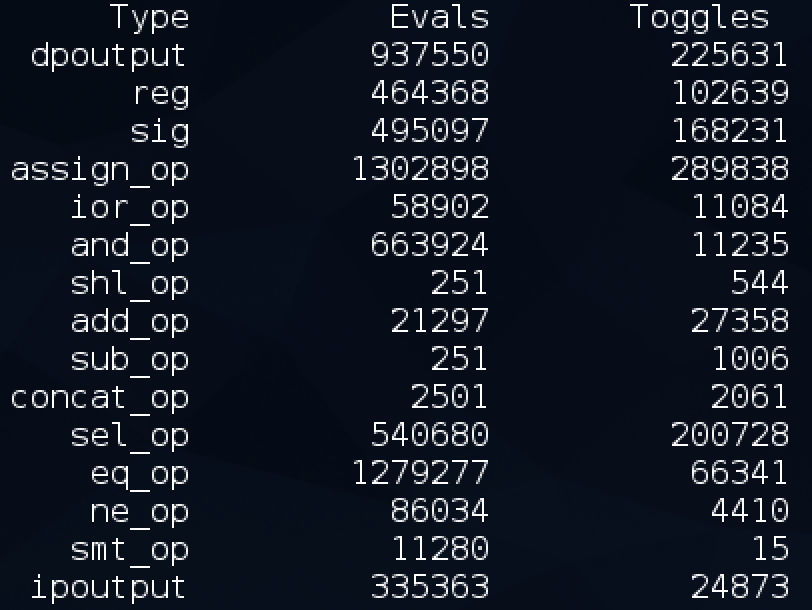
\includegraphics[width=0.7\textwidth]{3Results/fig/Toggles.png}
    \caption{Analyze output from Gezel using toggle alledge option.}
    \label{fig:toggles}
\end{figure}

The total activity (numbers of bits flipped) is 168231 for the complete set of 250 data points. According to Landauer's principle\footnote{\url{https://en.wikipedia.org/wiki/Landauer's_principle}} the minimum possible energy used to toggle a bit follows the second law of thermodynamics. At room temperature the minimum energy for flipping a bit is approximately $kT \ln(2) \approx 2.75 \times 10^{-21}$ J. Since toggling a bit counts as erasing information, the entropy must be maintained as the manifestation of heat. \\
\\
However, Laundauer's principle is not a very good estimation for the actual energy used per toggle. Looking at a standard modern transistor\footnote{\url{https://en.wikipedia.org/wiki/Transistor-transistor_logic}} we get a value of 100 pJ per bit flip, approximately $3.6 \times 10^{10}$ times larger than the result from Landauer's principle.
This is a more reasonable value since processors are built from real transistors and not theoretically-minimum devices. \\
\\
The energy used for applying the moving window integration filter on 250 data points is then $168231 \times 100$ pJ $\approx 17$ \si{\micro}{J}. \\
\\
We must bear in mind that energy also unavoidably dissipates from wires. When implementing the filters in hardware but keeping data acquisition and peak detection in software, the communication between software and hardware also costs energy since it may involve converting signals (and thus flipping bits).

\subsubsection{CPU speed}
\label{sec:cpuSpeed}

We check the hardware simulation in GKTwave, a tool for visualizing concurrent values in registers and signals.\\

\textbf{Total clock cycles:} It takes 8760 clock cycles to calculate the 250 data points. It costs an additional 2270 clock cycles if the resulting data is saved in memory using the \texttt{BUS} after each computation. The result is a total of 11030 clock cycles for the complete data set. \\

\textbf{Typical data point:} Checking the amount of clock cycles for a typical data point (complete loop in the program), we get 44 cycles. \\

\textbf{Average data point:} If we calculate the average amount of clock cycles pr data point, we get: $\frac{11030}{250} = 44.12$ clock cycles, meaning that on average all data points take the same amount of clock cycles, and therefore time. This is a nice result from bit shifting instead if integer division; while division may take few or many clock cycles (depending on the numbers $A$ and $B$ in $\frac{A}{B}$), bit shifting is consistent. \\

\textbf{Length of clock cycle:} Gezel does not tell time. Since we are limited in data regarding the length of a clock cycle, we make do with the example from lecture 9. We assume that a read/write action takes 25 ns, and an \texttt{ALU} computation takes 50 ns. In order to find the proper period we must identify the critical path for the CPU. Looking at figure \ref{fig:ComArch} or appendix \ref{app:ComArch}, we see that the critical path is:

\begin{center} 
$\texttt{REG} \rightarrow \texttt{ALU} \rightarrow \texttt{MUX} \rightarrow \texttt{REG}.$
\end{center}

\textbf{Computation time:} This leaves us with a clock period of 25 ns + 50 ns + 25 ns = 100 ns, assuming that the time through the \texttt{MUX} is negligible. With this time per clock cycle, we get that the time per data point is $44 \times 100$ ns = 4.4 \si{\micro}{s}. The 10000 data points from assignment 1 would then take 10000 $\times$ 4.4 \si{\micro}{s} = 44 ms of computation time.\\

\textbf{Clock rate:} With a clock period of 100 ns, we get a frequency of $\frac{1}{100 \text{ ns}} = 10$ MHz. \\

This computation time is much higher than in assignment 1. In our C program, the total computation time was 5.4 ms for applying all filters. The moving window integration filter took up 75 \%, i.e. 4 ms.\\

However: The computation time in C was recorded using a modern day CPU with a processor clock rate of 2.7 GHz, 270 times faster than the CPU for the hardware implementation.\\

With this adjustment, the relative time for the software implementation is 4 ms $\times$ 270 = 1080 ms. This gives the hardware implementation (by rough estimation) the capacity of being $\frac{1080 \text{ ms}}{44 \text{ ms}} = 24.5 \approx 25$ times faster. \\

\subsubsection{CPU area}
\label{sec:cpuArea}

A total sum of all registers and signals used in the CPU (not counting the \texttt{BUS}) is calculated and shown in table \ref{tabel:areaSum}:

\begin{table}[H]
\begin{center}
    \begin{tabular}{|l|l|l|}
    \hline
    \textbf{Datapath}                          & \textbf{Category}   & \textbf{Total bit amount (size)}                       \\ \hline
    \texttt{PC}                                 & Registers & 5                                \\
    ~                                  & Signals   & 5                                \\ \hline
    \texttt{ROM}                                & $-$       & 0                                \\ \hline
    \texttt{fetch}\footnote{See CPU code}                              & $-$       & 0                                \\ \hline
    \texttt{REG}                                & Registers & 7 $\cdot$ 32 \\ \hline
    \texttt{ALU}                                & Signals   & 8                                \\ \hline
    \texttt{CONTROL}                            & $-$       & 0                                \\ \hline
    \texttt{SHUTTLE}                            & $-$       & 0                                \\ \hline
    \texttt{MUX}                                & $-$       & 0                                \\ \hline \hline
    \textbf{Signals between datapaths}  & Signals   & 8 + 5 + 16 + 5 $\cdot$ 32 + 2 $\cdot$ 4          \\ \hline \hline
    \textbf{From fetch to \texttt{ROM}} & Signals   & 5 + 1 +  2 $\cdot$ 16                    \\ \hline \hline
    ~                                  & TOTAL SUM & 477                              \\ \hline
    \end{tabular}
    \caption{Sum of all signals and register in the CPU (not counting the \texttt{BUS}).}
    \label{tabel:areaSum}
    \end{center}
\end{table}

We only define 7 registers in Gezel: R1 through R7. R0 is not defined directly. If a component asks for the value in R0 (or rather: if the selectors sent to \texttt{REG} are not in the interval 1-7), \texttt{REG} just outputs the value 0. Hence we may think of R0 as a pseudo register.\\

The datapaths \texttt{ROM}, \texttt{CONTROL}, \texttt{SHUTTLE}, and \texttt{MUX} in Gezel do not contain any internal registers or signals. All signals between datapaths are counted in the separate category \textit{Signals between datapaths}.\\

With an overall size of around 480 bits, we reckon this is a small footprint, compared to other standard CPUs with often millions of transistors (and hence bits).\footnote{https://en.wikipedia.org/wiki/Transistor_count}